\documentclass[a4paper, oneside, final]{scrartcl}

\usepackage[spanish]{babel}
\usepackage{scrlayer-scrpage}
\usepackage{titlesec}
\usepackage{anysize}
\usepackage{marvosym}
\usepackage{tabularx,colortbl}
\usepackage{ebgaramond}
\usepackage{microtype}
\usepackage{bera}
\usepackage{listings}
\usepackage{xcolor}
\usepackage{hyperref}
\usepackage{graphicx}
\usepackage{amsmath}
\usepackage{cite}

\titleformat{\section}{\large\scshape\raggedright}{}{0em}{}[\titlerule]

\pagestyle{scrheadings}

\addtolength{\voffset}{-0.5in}
\addtolength{\textheight}{3cm}

\newcommand{\gray}{\rowcolor[gray]{.90}}

\renewcommand{\headfont}{\normalfont\rmfamily}

\marginsize{2cm}{2cm}{2cm}{2cm}
\setlength{\parindent}{0cm}

\colorlet{punct}{red!60!black}
\definecolor{background}{HTML}{EEEEEE}
\definecolor{delim}{RGB}{20,105,176}
\colorlet{numb}{magenta!60!black}

\lstdefinelanguage{json}{
    basicstyle=\normalfont\ttfamily,
    numbers=left,
    numberstyle=\scriptsize,
    stepnumber=1,
    numbersep=8pt,
    showstringspaces=false,
    breaklines=true,
    frame=lines,
    backgroundcolor=\color{background},
    literate=
     *{0}{{{\color{numb}0}}}{1}
      {1}{{{\color{numb}1}}}{1}
      {2}{{{\color{numb}2}}}{1}
      {3}{{{\color{numb}3}}}{1}
      {4}{{{\color{numb}4}}}{1}
      {5}{{{\color{numb}5}}}{1}
      {6}{{{\color{numb}6}}}{1}
      {7}{{{\color{numb}7}}}{1}
      {8}{{{\color{numb}8}}}{1}
      {9}{{{\color{numb}9}}}{1}
      {:}{{{\color{punct}{:}}}}{1}
      {,}{{{\color{punct}{,}}}}{1}
      {\{}{{{\color{delim}{\{}}}}{1}
      {\}}{{{\color{delim}{\}}}}}{1}
      {[}{{{\color{delim}{[}}}}{1}
      {]}{{{\color{delim}{]}}}}{1},
}

\begin{document}

\thispagestyle{empty}

\begin{center}
    %\newcommand{\HRule}{\rule{\linewidth}{0.5mm}}
    \begin{minipage}{0.29\textwidth} 
        \center{
\includegraphics[scale = 0.06]{images/logo_unam.png}}
    \end{minipage}
    \begin{minipage}{0.40\textwidth} 
    \center{\textsc{\LARGE Universidad Nacional \\[5mm] Autónoma de México}}\\
    \end{minipage}
    \begin{minipage}{0.29\textwidth}
        \center{
\includegraphics[scale =0.18]{images/logo_ciencias.png}}
    \end{minipage}
    \vspace{5mm}					
    
    \textsc{\noindent \LARGE Facultad de Ciencias}\\[20mm]
    
    \textsc{\LARGE   Ingeniería de Software \\[5mm]
                    \LARGE 2024-2}      \\[20mm]
    
    \textsc{\textbf{\huge   Análisis de requerimientos}}\\[5mm]
    \textsc{\LARGE  Pizarra colaborativa para computólogos}\\[20mm]

    \LARGE
    \textsc{Equipo I}\\[5mm]
    \Large 
    \textsc{Diego Sebastián Sánchez Correa}\\[2mm]
    \textsc{Mauro Emiliano Chávez Zamora}\\[2mm]
    \textsc{Ulises Josué Anaya Pérez}\\[2mm]
    \textsc{Daniel Linares Gil} \\[2mm]
    \textsc{Karyme Ivette Azpeitia García}
    \\[20mm]

    \large Creado: 15/02/2024\\[2mm]
    \large Última actualización: 20/02/2024\\
    
\end{center}	
\newpage  


\section{Objetivo}

El objetivo de este documento es diseñar una aplicación web para la creación y edición de pizarras que permita la colaboración entre usuarios en tiempo real.


\section{Entidad relación}

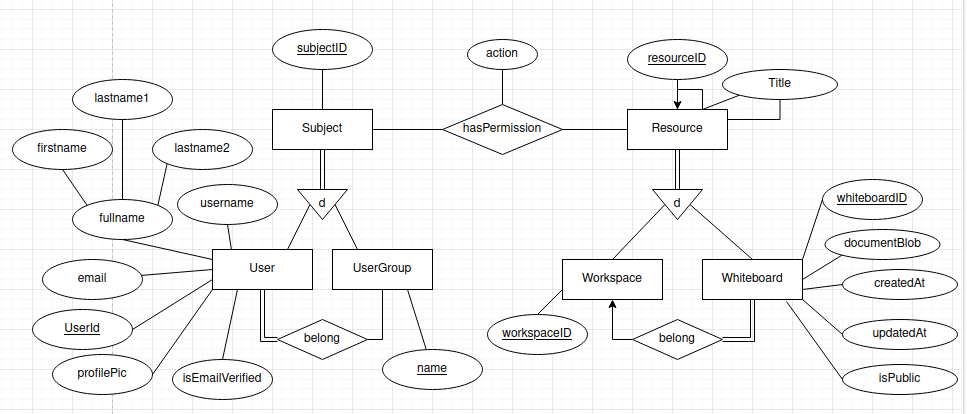
\includegraphics[width=\textwidth]{images/EntidadRelacion.png}

\section{Modelo Relacional}
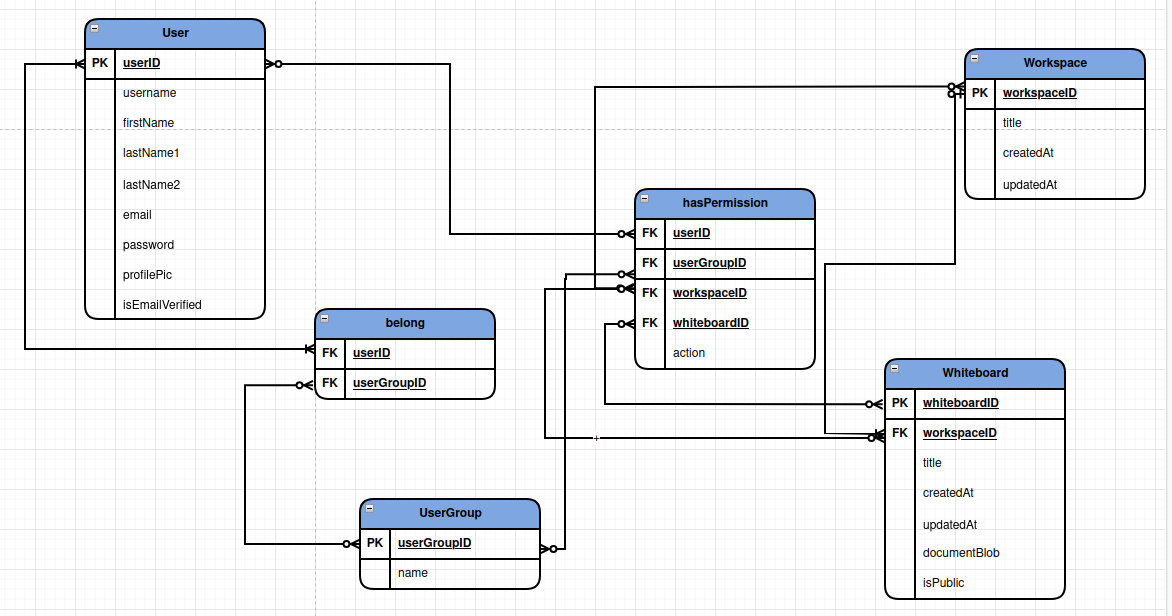
\includegraphics[width=\textwidth]{images/Relacional.png}

\section{Mockups Pizarra}
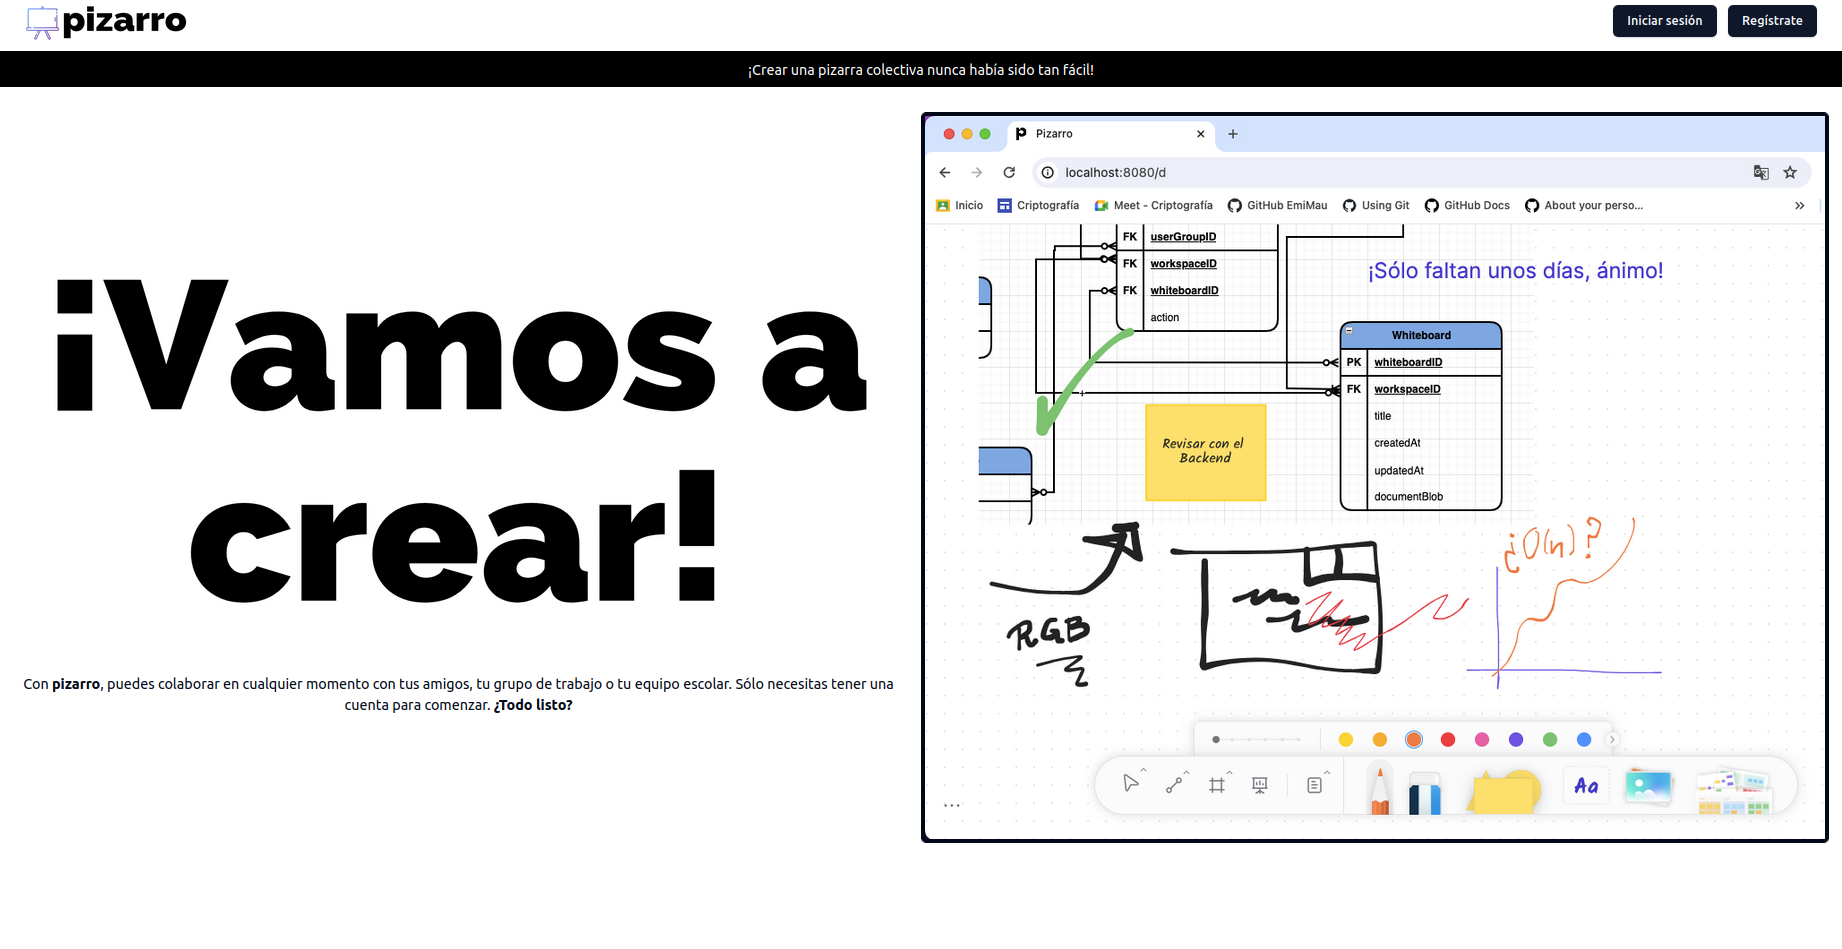
\includegraphics[width= \textwidth]{images/mock0.png}
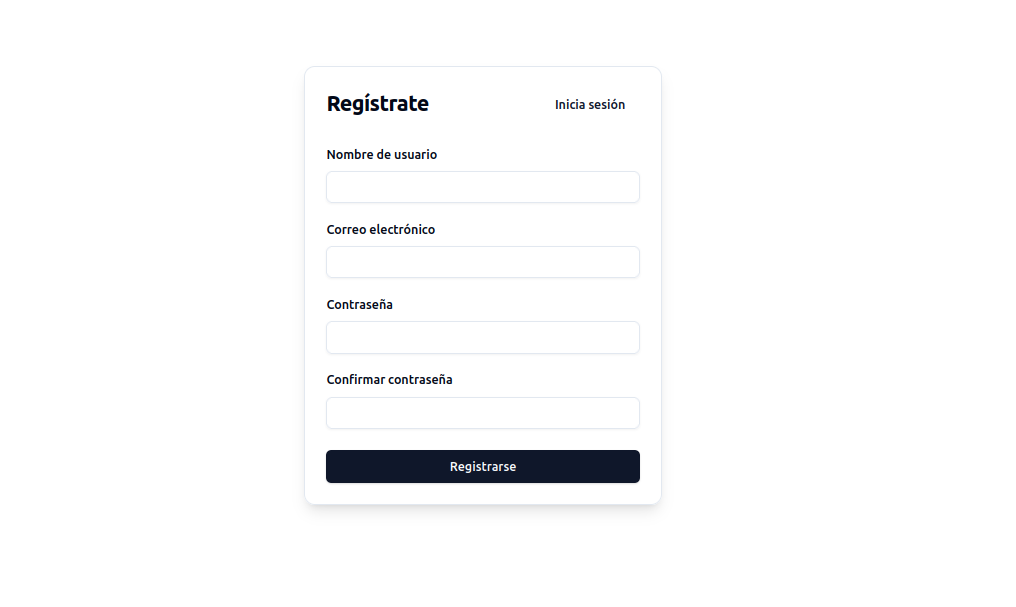
\includegraphics[width= \textwidth]{images/mock01.png} \\
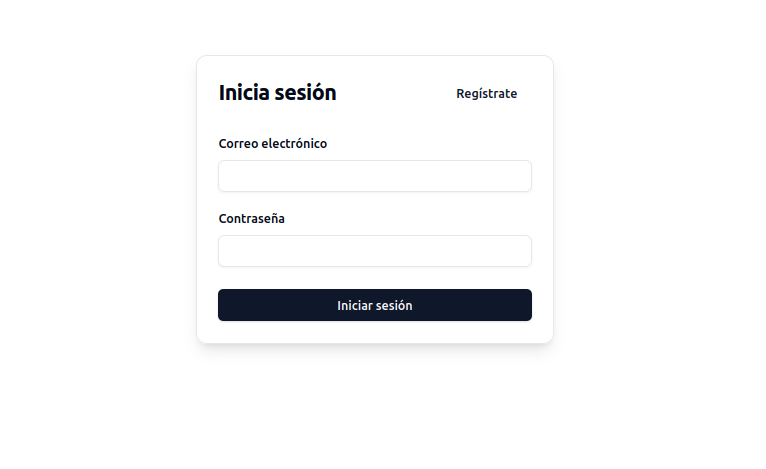
\includegraphics[width= \textwidth]{images/mock02.png} \\



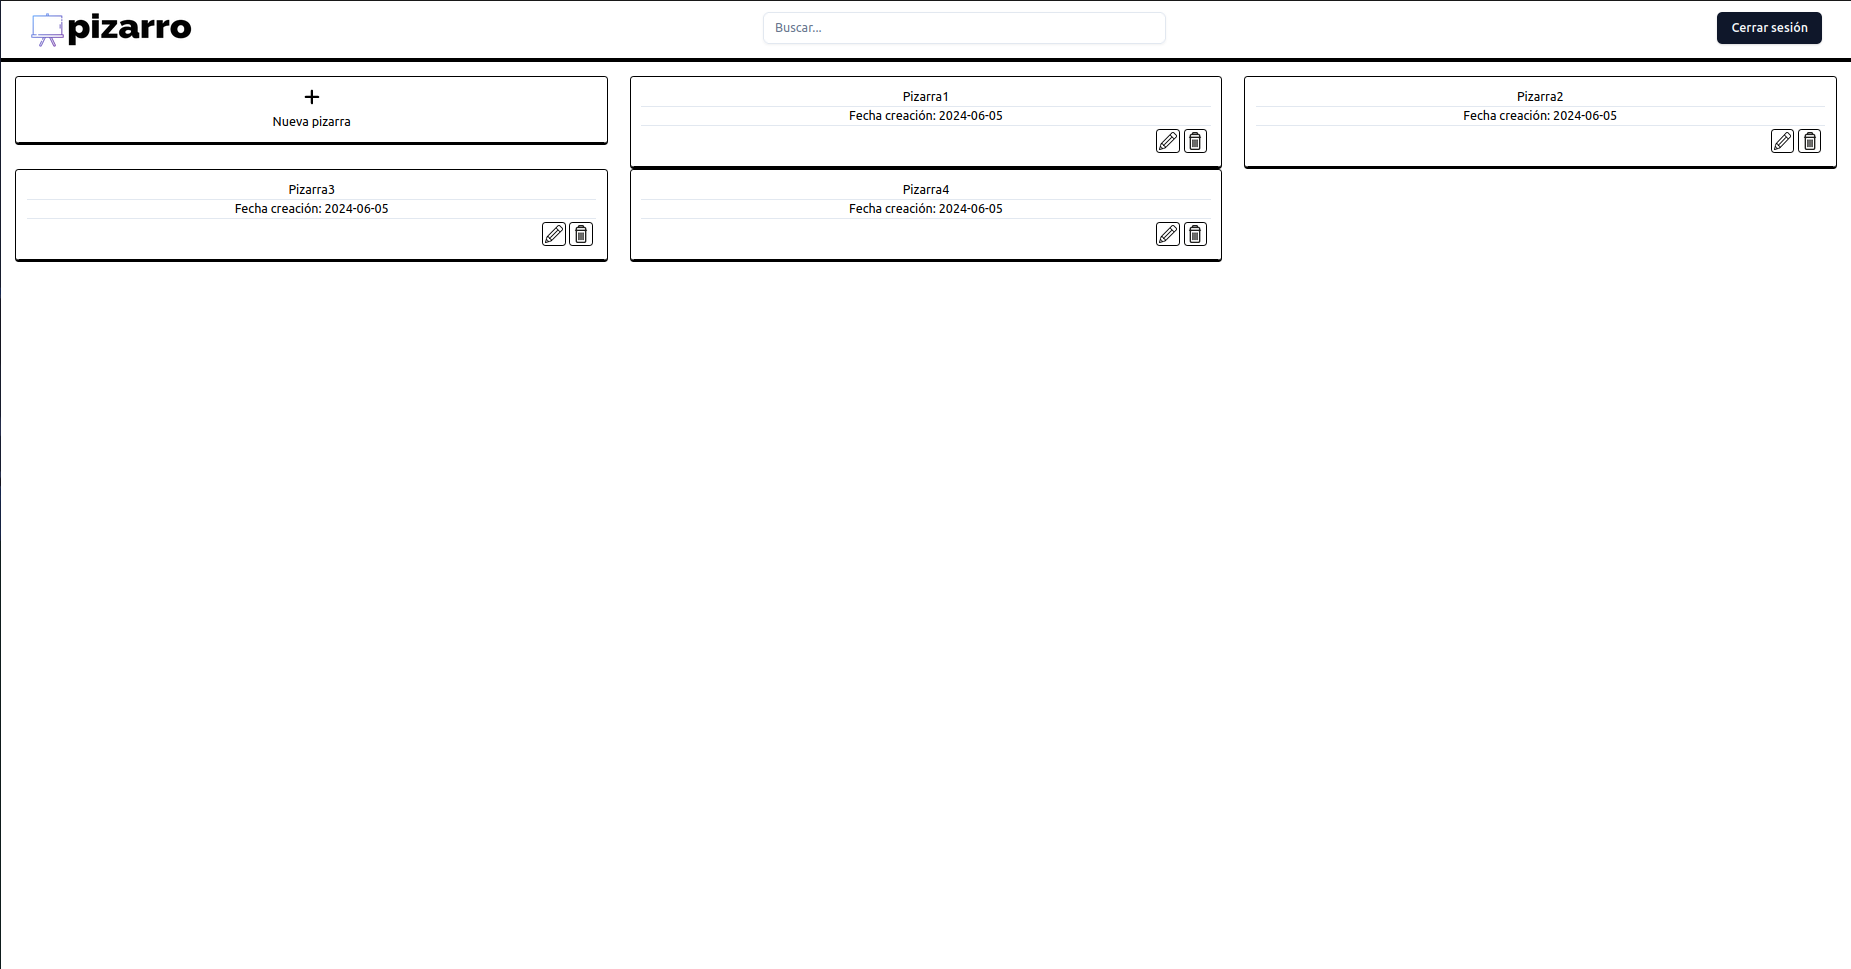
\includegraphics[width= \textwidth]{images/mock1.png} \\
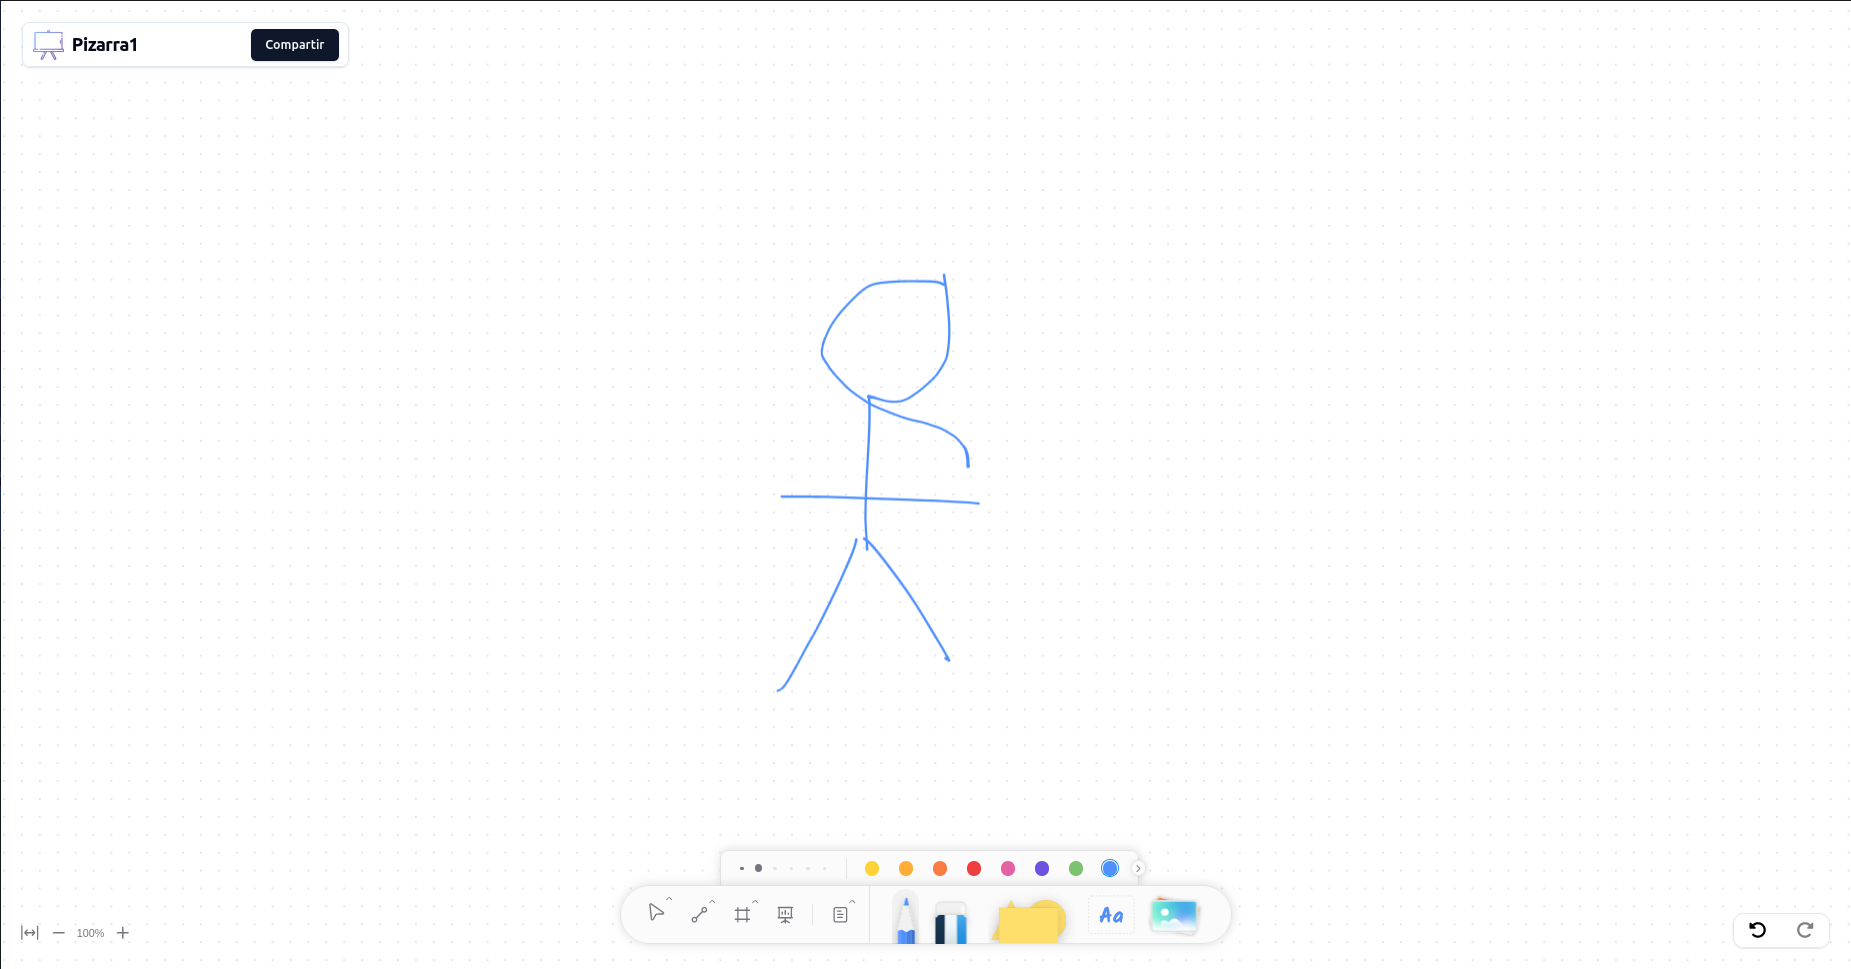
\includegraphics[width= \textwidth]{images/mock2.png}
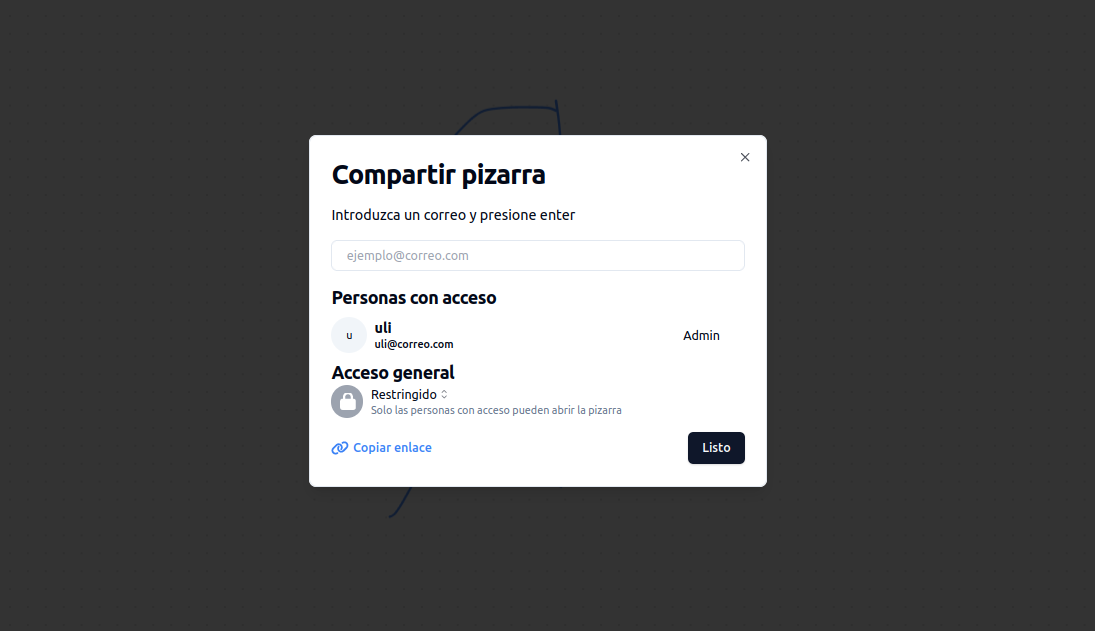
\includegraphics[width= \textwidth]{images/Mock.png}


\clearpage

\section{Casos de Uso}

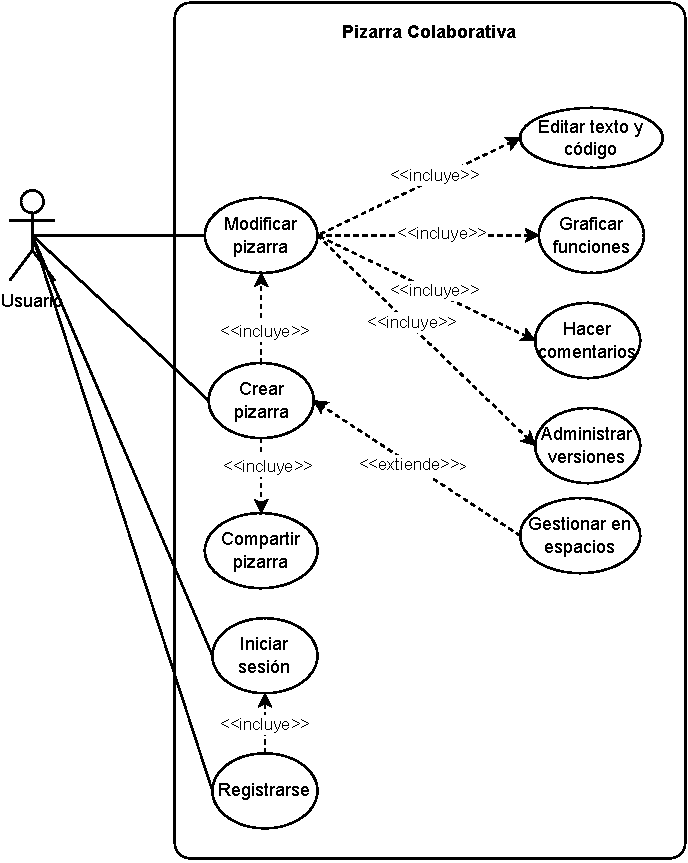
\includegraphics[width=\textwidth]{images/Casos-de-uso-1.pdf}

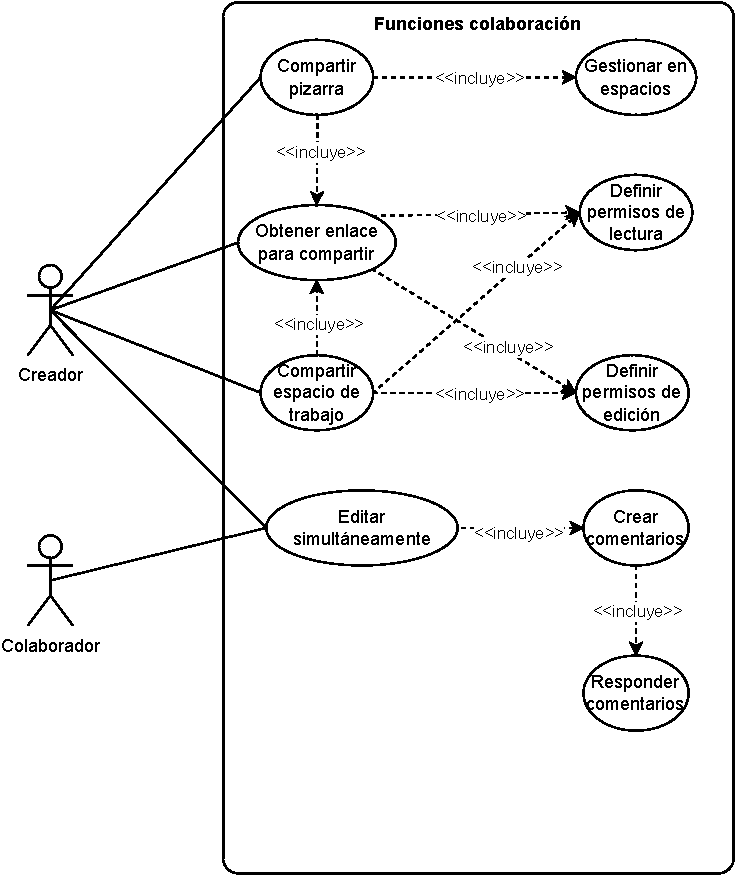
\includegraphics[width=\textwidth]{images/Casos-de-uso-2.pdf}

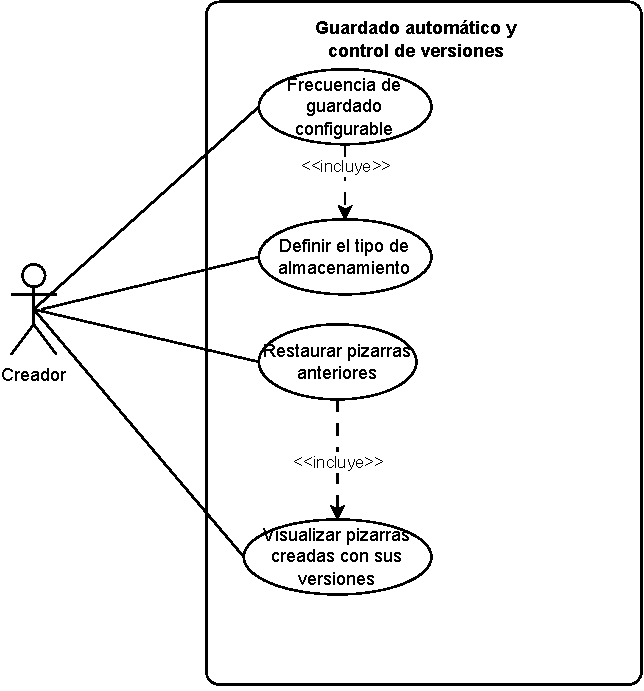
\includegraphics[width=\textwidth]{images/Casos-de-uso-3.pdf}

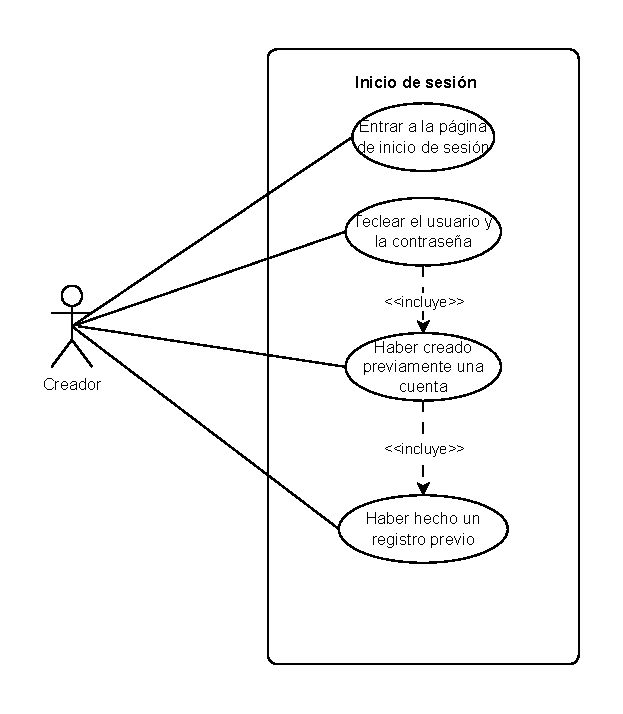
\includegraphics[width=\textwidth]{images/CasoUso4-1.pdf}
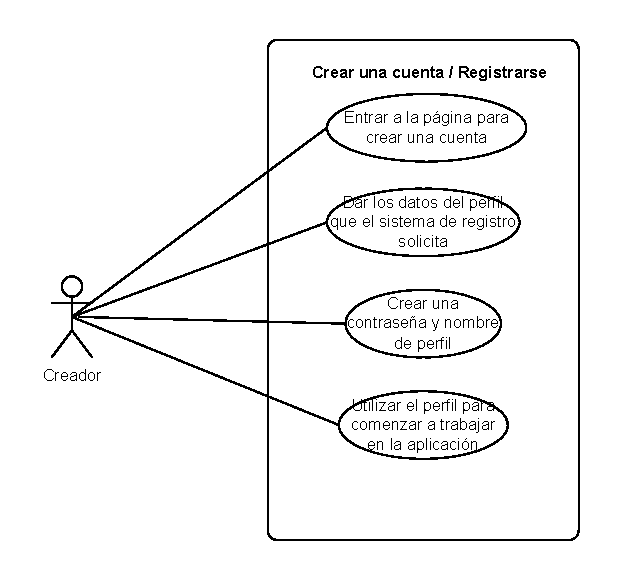
\includegraphics[width=\textwidth]{images/CasoUso5.pdf}

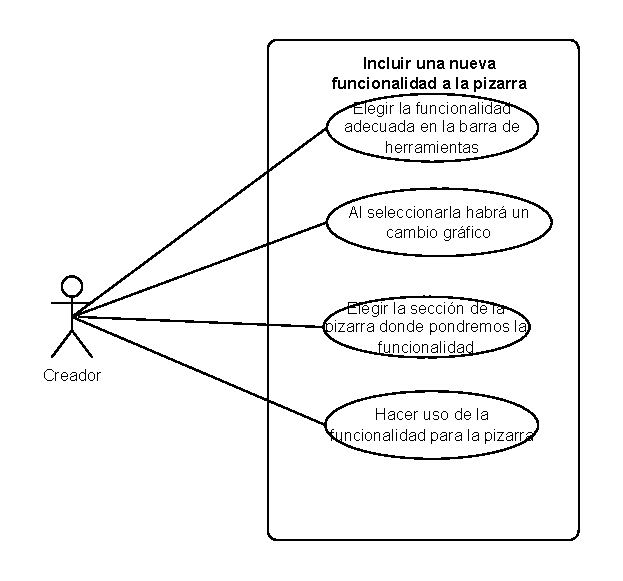
\includegraphics[width=\textwidth]{images/CasoUso6.pdf}
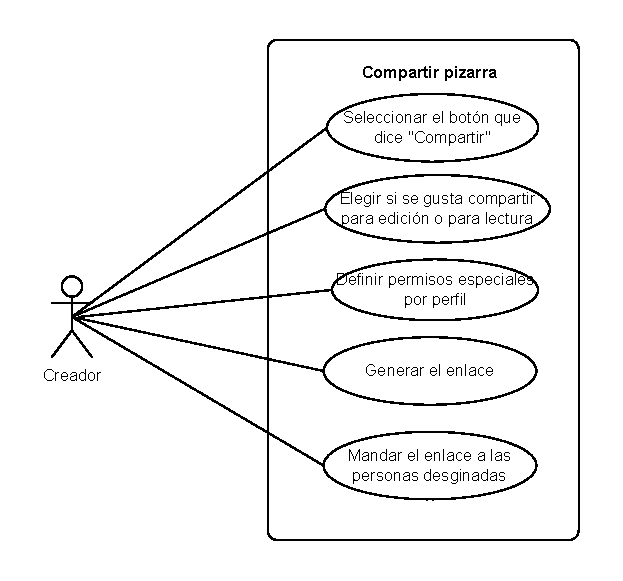
\includegraphics[width=\textwidth]{images/CasoUso7.pdf}





\bibliographystyle{plain}
\end{document}